\documentclass[1p]{elsarticle_modified}
%\bibliographystyle{elsarticle-num}

%\usepackage[colorlinks]{hyperref}
%\usepackage{abbrmath_seonhwa} %\Abb, \Ascr, \Acal ,\Abf, \Afrak
\usepackage{amsfonts}
\usepackage{amssymb}
\usepackage{amsmath}
\usepackage{amsthm}
\usepackage{scalefnt}
\usepackage{amsbsy}
\usepackage{kotex}
\usepackage{caption}
\usepackage{subfig}
\usepackage{color}
\usepackage{graphicx}
\usepackage{xcolor} %% white, black, red, green, blue, cyan, magenta, yellow
\usepackage{float}
\usepackage{setspace}
\usepackage{hyperref}

\usepackage{tikz}
\usetikzlibrary{arrows}

\usepackage{multirow}
\usepackage{array} % fixed length table
\usepackage{hhline}

%%%%%%%%%%%%%%%%%%%%%
\makeatletter
\renewcommand*\env@matrix[1][\arraystretch]{%
	\edef\arraystretch{#1}%
	\hskip -\arraycolsep
	\let\@ifnextchar\new@ifnextchar
	\array{*\c@MaxMatrixCols c}}
\makeatother %https://tex.stackexchange.com/questions/14071/how-can-i-increase-the-line-spacing-in-a-matrix
%%%%%%%%%%%%%%%

\usepackage[normalem]{ulem}

\newcommand{\msout}[1]{\ifmmode\text{\sout{\ensuremath{#1}}}\else\sout{#1}\fi}
%SOURCE: \msout is \stkout macro in https://tex.stackexchange.com/questions/20609/strikeout-in-math-mode

\newcommand{\cancel}[1]{
	\ifmmode
	{\color{red}\msout{#1}}
	\else
	{\color{red}\sout{#1}}
	\fi
}

\newcommand{\add}[1]{
	{\color{blue}\uwave{#1}}
}

\newcommand{\replace}[2]{
	\ifmmode
	{\color{red}\msout{#1}}{\color{blue}\uwave{#2}}
	\else
	{\color{red}\sout{#1}}{\color{blue}\uwave{#2}}
	\fi
}

\newcommand{\Sol}{\mathcal{S}} %segment
\newcommand{\D}{D} %diagram
\newcommand{\A}{\mathcal{A}} %arc


%%%%%%%%%%%%%%%%%%%%%%%%%%%%%5 test

\def\sl{\operatorname{\textup{SL}}(2,\Cbb)}
\def\psl{\operatorname{\textup{PSL}}(2,\Cbb)}
\def\quan{\mkern 1mu \triangleright \mkern 1mu}

\theoremstyle{definition}
\newtheorem{thm}{Theorem}[section]
\newtheorem{prop}[thm]{Proposition}
\newtheorem{lem}[thm]{Lemma}
\newtheorem{ques}[thm]{Question}
\newtheorem{cor}[thm]{Corollary}
\newtheorem{defn}[thm]{Definition}
\newtheorem{exam}[thm]{Example}
\newtheorem{rmk}[thm]{Remark}
\newtheorem{alg}[thm]{Algorithm}

\newcommand{\I}{\sqrt{-1}}
\begin{document}

%\begin{frontmatter}
%
%\title{Boundary parabolic representations of knots up to 8 crossings}
%
%%% Group authors per affiliation:
%\author{Yunhi Cho} 
%\address{Department of Mathematics, University of Seoul, Seoul, Korea}
%\ead{yhcho@uos.ac.kr}
%
%
%\author{Seonhwa Kim} %\fnref{s_kim}}
%\address{Center for Geometry and Physics, Institute for Basic Science, Pohang, 37673, Korea}
%\ead{ryeona17@ibs.re.kr}
%
%\author{Hyuk Kim}
%\address{Department of Mathematical Sciences, Seoul National University, Seoul 08826, Korea}
%\ead{hyukkim@snu.ac.kr}
%
%\author{Seokbeom Yoon}
%\address{Department of Mathematical Sciences, Seoul National University, Seoul, 08826,  Korea}
%\ead{sbyoon15@snu.ac.kr}
%
%\begin{abstract}
%We find all boundary parabolic representation of knots up to 8 crossings.
%
%\end{abstract}
%\begin{keyword}
%    \MSC[2010] 57M25 
%\end{keyword}
%
%\end{frontmatter}

%\linenumbers
%\tableofcontents
%
\newcommand\colored[1]{\textcolor{white}{\rule[-0.35ex]{0.8em}{1.4ex}}\kern-0.8em\color{red} #1}%
%\newcommand\colored[1]{\textcolor{white}{ #1}\kern-2.17ex	\textcolor{white}{ #1}\kern-1.81ex	\textcolor{white}{ #1}\kern-2.15ex\color{red}#1	}

{\Large $\underline{12n_{0856}~(K12n_{0856})}$}

\setlength{\tabcolsep}{10pt}
\renewcommand{\arraystretch}{1.6}
\vspace{1cm}\begin{tabular}{m{100pt}>{\centering\arraybackslash}m{274pt}}
\multirow{5}{120pt}{
	\centering
	\includegraphics[width=112pt]{../../../GIT/diagram.site/Diagrams/png/2945_12n_0856.png}\\
\ \ \ A knot diagram\footnotemark}&
\allowdisplaybreaks
\textbf{Linearized knot diagam} \\
\cline{2-2}
 &
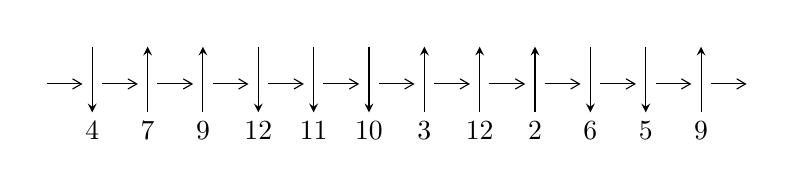
\begin{tikzpicture}[x=20pt, y=17pt]
	% nodes
	\node (C0) at (0, 0) {};
	\node (C1) at (1, 0) {};
	\node (C1U) at (1, +1) {};
	\node (C1D) at (1, -1) {4};

	\node (C2) at (2, 0) {};
	\node (C2U) at (2, +1) {};
	\node (C2D) at (2, -1) {7};

	\node (C3) at (3, 0) {};
	\node (C3U) at (3, +1) {};
	\node (C3D) at (3, -1) {9};

	\node (C4) at (4, 0) {};
	\node (C4U) at (4, +1) {};
	\node (C4D) at (4, -1) {12};

	\node (C5) at (5, 0) {};
	\node (C5U) at (5, +1) {};
	\node (C5D) at (5, -1) {11};

	\node (C6) at (6, 0) {};
	\node (C6U) at (6, +1) {};
	\node (C6D) at (6, -1) {10};

	\node (C7) at (7, 0) {};
	\node (C7U) at (7, +1) {};
	\node (C7D) at (7, -1) {3};

	\node (C8) at (8, 0) {};
	\node (C8U) at (8, +1) {};
	\node (C8D) at (8, -1) {12};

	\node (C9) at (9, 0) {};
	\node (C9U) at (9, +1) {};
	\node (C9D) at (9, -1) {2};

	\node (C10) at (10, 0) {};
	\node (C10U) at (10, +1) {};
	\node (C10D) at (10, -1) {6};

	\node (C11) at (11, 0) {};
	\node (C11U) at (11, +1) {};
	\node (C11D) at (11, -1) {5};

	\node (C12) at (12, 0) {};
	\node (C12U) at (12, +1) {};
	\node (C12D) at (12, -1) {9};
	\node (C13) at (13, 0) {};

	% arrows
	\draw[->,>={angle 60}]
	(C0) edge (C1) (C1) edge (C2) (C2) edge (C3) (C3) edge (C4) (C4) edge (C5) (C5) edge (C6) (C6) edge (C7) (C7) edge (C8) (C8) edge (C9) (C9) edge (C10) (C10) edge (C11) (C11) edge (C12) (C12) edge (C13) ;	\draw[->,>=stealth]
	(C1U) edge (C1D) (C2D) edge (C2U) (C3D) edge (C3U) (C4U) edge (C4D) (C5U) edge (C5D) (C6U) edge (C6D) (C7D) edge (C7U) (C8D) edge (C8U) (C9D) edge (C9U) (C10U) edge (C10D) (C11U) edge (C11D) (C12D) edge (C12U) ;
	\end{tikzpicture} \\
\hhline{~~} \\& 
\textbf{Solving Sequence} \\ \cline{2-2} 
 &
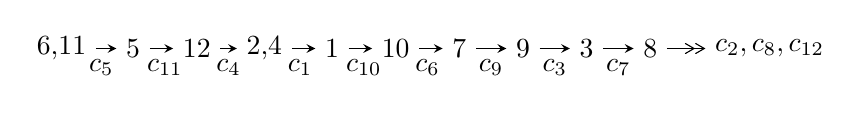
\begin{tikzpicture}[x=23pt, y=7pt]
	% node
	\node (A0) at (-1/8, 0) {6,11};
	\node (A1) at (1, 0) {5};
	\node (A2) at (2, 0) {12};
	\node (A3) at (49/16, 0) {2,4};
	\node (A4) at (33/8, 0) {1};
	\node (A5) at (41/8, 0) {10};
	\node (A6) at (49/8, 0) {7};
	\node (A7) at (57/8, 0) {9};
	\node (A8) at (65/8, 0) {3};
	\node (A9) at (73/8, 0) {8};
	\node (C1) at (1/2, -1) {$c_{5}$};
	\node (C2) at (3/2, -1) {$c_{11}$};
	\node (C3) at (5/2, -1) {$c_{4}$};
	\node (C4) at (29/8, -1) {$c_{1}$};
	\node (C5) at (37/8, -1) {$c_{10}$};
	\node (C6) at (45/8, -1) {$c_{6}$};
	\node (C7) at (53/8, -1) {$c_{9}$};
	\node (C8) at (61/8, -1) {$c_{3}$};
	\node (C9) at (69/8, -1) {$c_{7}$};
	\node (A10) at (11, 0) {$c_{2},c_{8},c_{12}$};

	% edge
	\draw[->,>=stealth]	
	(A0) edge (A1) (A1) edge (A2) (A2) edge (A3) (A3) edge (A4) (A4) edge (A5) (A5) edge (A6) (A6) edge (A7) (A7) edge (A8) (A8) edge (A9) ;
	\draw[->>,>={angle 60}]	
	(A9) edge (A10);
\end{tikzpicture} \\ 

\end{tabular} \\

\footnotetext{
The image of knot diagram is generated by the software ``\textbf{Draw programme}" developed by Andrew Bartholomew(\url{http://www.layer8.co.uk/maths/draw/index.htm\#Running-draw}), where we modified some parts for our purpose(\url{https://github.com/CATsTAILs/LinksPainter}).
}\phantom \\ \newline 
\centering \textbf{Ideals for irreducible components\footnotemark of $X_{\text{par}}$} 
 
\begin{align*}
I^u_{1}&=\langle 
- u^{15}-5 u^{14}+\cdots+2 b-4,\;- u^{15}-4 u^{14}+\cdots+2 a+1,\;u^{16}+5 u^{15}+\cdots+30 u+4\rangle \\
I^u_{2}&=\langle 
-74 u^4 a^3+62 u^4 a^2+\cdots+20 a-170,\;2 u^4 a^3-11 u^4 a+\cdots-23 a-23,\;u^5- u^4+4 u^3-3 u^2+3 u-1\rangle \\
I^u_{3}&=\langle 
- u^5- u^4-3 u^3-3 u^2+b- u-1,\;u^8+7 u^6- u^5+15 u^4-4 u^3+10 u^2+a-4 u+2,\\
\phantom{I^u_{3}}&\phantom{= \langle  }u^9+7 u^7+16 u^5+13 u^3+3 u+1\rangle \\
\\
\end{align*}
\raggedright * 3 irreducible components of $\dim_{\mathbb{C}}=0$, with total 45 representations.\\
\footnotetext{All coefficients of polynomials are rational numbers. But the coefficients are sometimes approximated in decimal forms when there is not enough margin.}
\newpage
\renewcommand{\arraystretch}{1}
\centering \section*{I. $I^u_{1}= \langle - u^{15}-5 u^{14}+\cdots+2 b-4,\;- u^{15}-4 u^{14}+\cdots+2 a+1,\;u^{16}+5 u^{15}+\cdots+30 u+4 \rangle$}
\flushleft \textbf{(i) Arc colorings}\\
\begin{tabular}{m{7pt} m{180pt} m{7pt} m{180pt} }
\flushright $a_{6}=$&$\begin{pmatrix}1\\0\end{pmatrix}$ \\
\flushright $a_{11}=$&$\begin{pmatrix}0\\u\end{pmatrix}$ \\
\flushright $a_{5}=$&$\begin{pmatrix}1\\- u^2\end{pmatrix}$ \\
\flushright $a_{12}=$&$\begin{pmatrix}- u\\u^3+u\end{pmatrix}$ \\
\flushright $a_{2}=$&$\begin{pmatrix}\frac{1}{2} u^{15}+2 u^{14}+\cdots-\frac{5}{2} u-\frac{1}{2}\\\frac{1}{2} u^{15}+\frac{5}{2} u^{14}+\cdots+\frac{25}{2} u+2\end{pmatrix}$ \\
\flushright $a_{4}=$&$\begin{pmatrix}u^2+1\\- u^4-2 u^2\end{pmatrix}$ \\
\flushright $a_{1}=$&$\begin{pmatrix}u^{15}+\frac{9}{2} u^{14}+\cdots+32 u+\frac{11}{2}\\\frac{1}{2} u^{15}+\frac{5}{2} u^{14}+\cdots+\frac{33}{2} u+2\end{pmatrix}$ \\
\flushright $a_{10}=$&$\begin{pmatrix}u\\u\end{pmatrix}$ \\
\flushright $a_{7}=$&$\begin{pmatrix}u^2+1\\u^2\end{pmatrix}$ \\
\flushright $a_{9}=$&$\begin{pmatrix}\frac{3}{4} u^{15}+\frac{13}{4} u^{14}+\cdots+\frac{89}{4} u+3\\-\frac{1}{2} u^{15}-\frac{5}{2} u^{14}+\cdots-\frac{41}{2} u-3\end{pmatrix}$ \\
\flushright $a_{3}=$&$\begin{pmatrix}- u^{15}-\frac{9}{2} u^{14}+\cdots-33 u-\frac{9}{2}\\-\frac{1}{2} u^{15}-\frac{5}{2} u^{14}+\cdots-\frac{31}{2} u-2\end{pmatrix}$ \\
\flushright $a_{8}=$&$\begin{pmatrix}\frac{1}{4} u^{15}+\frac{3}{4} u^{14}+\cdots-\frac{33}{4} u-1\\-\frac{1}{2} u^{15}-\frac{5}{2} u^{14}+\cdots-\frac{39}{2} u-3\end{pmatrix}$\\&\end{tabular}
\flushleft \textbf{(ii) Obstruction class $= -1$}\\~\\
\flushleft \textbf{(iii) Cusp Shapes $= - u^{15}-5 u^{14}-23 u^{13}-70 u^{12}-184 u^{11}-388 u^{10}-709 u^9-1086 u^8-1443 u^7-1613 u^6-1539 u^5-1210 u^4-775 u^3-384 u^2-138 u-26$}\\~\\
\newpage\renewcommand{\arraystretch}{1}
\flushleft \textbf{(iv) u-Polynomials at the component}\newline \\
\begin{tabular}{m{50pt}|m{274pt}}
Crossings & \hspace{64pt}u-Polynomials at each crossing \\
\hline $$\begin{aligned}c_{1}\end{aligned}$$&$\begin{aligned}
&u^{16}-15 u^{15}+\cdots-128 u+32
\end{aligned}$\\
\hline $$\begin{aligned}c_{2},c_{7},c_{9}\end{aligned}$$&$\begin{aligned}
&u^{16}+u^{15}+\cdots-3 u^2+1
\end{aligned}$\\
\hline $$\begin{aligned}c_{3},c_{8},c_{12}\end{aligned}$$&$\begin{aligned}
&u^{16}+10 u^{14}+\cdots- u+1
\end{aligned}$\\
\hline $$\begin{aligned}c_{4},c_{5},c_{6}\\c_{10},c_{11}\end{aligned}$$&$\begin{aligned}
&u^{16}+5 u^{15}+\cdots+30 u+4
\end{aligned}$\\
\hline
\end{tabular}\\~\\
\newpage\renewcommand{\arraystretch}{1}
\flushleft \textbf{(v) Riley Polynomials at the component}\newline \\
\begin{tabular}{m{50pt}|m{274pt}}
Crossings & \hspace{64pt}Riley Polynomials at each crossing \\
\hline $$\begin{aligned}c_{1}\end{aligned}$$&$\begin{aligned}
&y^{16}-7 y^{15}+\cdots+13824 y+1024
\end{aligned}$\\
\hline $$\begin{aligned}c_{2},c_{7},c_{9}\end{aligned}$$&$\begin{aligned}
&y^{16}-13 y^{15}+\cdots-6 y+1
\end{aligned}$\\
\hline $$\begin{aligned}c_{3},c_{8},c_{12}\end{aligned}$$&$\begin{aligned}
&y^{16}+20 y^{15}+\cdots+25 y+1
\end{aligned}$\\
\hline $$\begin{aligned}c_{4},c_{5},c_{6}\\c_{10},c_{11}\end{aligned}$$&$\begin{aligned}
&y^{16}+21 y^{15}+\cdots+116 y+16
\end{aligned}$\\
\hline
\end{tabular}\\~\\
\newpage\flushleft \textbf{(vi) Complex Volumes and Cusp Shapes}
$$\begin{array}{c|c|c}  
\text{Solutions to }I^u_{1}& \I (\text{vol} + \sqrt{-1}CS) & \text{Cusp shape}\\
 \hline 
\begin{aligned}
u &= -0.623980 + 0.651550 I \\
a &= -0.423845 - 0.017311 I \\
b &= \phantom{-}0.571868 + 0.505425 I\end{aligned}
 & -1.44391 - 0.70743 I & \phantom{-}3.72290 + 0.24608 I \\ \hline\begin{aligned}
u &= -0.623980 - 0.651550 I \\
a &= -0.423845 + 0.017311 I \\
b &= \phantom{-}0.571868 - 0.505425 I\end{aligned}
 & -1.44391 + 0.70743 I & \phantom{-}3.72290 - 0.24608 I \\ \hline\begin{aligned}
u &= -0.463938 + 1.039450 I \\
a &= \phantom{-}0.077415 + 0.436847 I \\
b &= \phantom{-}0.01364 + 1.74946 I\end{aligned}
 & \phantom{-}1.07382 + 9.25014 I & \phantom{-}4.41993 - 6.63902 I \\ \hline\begin{aligned}
u &= -0.463938 - 1.039450 I \\
a &= \phantom{-}0.077415 - 0.436847 I \\
b &= \phantom{-}0.01364 - 1.74946 I\end{aligned}
 & \phantom{-}1.07382 - 9.25014 I & \phantom{-}4.41993 + 6.63902 I \\ \hline\begin{aligned}
u &= -0.740661 + 0.206858 I \\
a &= \phantom{-}1.043460 + 0.692415 I \\
b &= -0.181803 - 0.371994 I\end{aligned}
 & -2.76230 + 5.19350 I & \phantom{-}1.00902 - 5.12835 I \\ \hline\begin{aligned}
u &= -0.740661 - 0.206858 I \\
a &= \phantom{-}1.043460 - 0.692415 I \\
b &= -0.181803 + 0.371994 I\end{aligned}
 & -2.76230 - 5.19350 I & \phantom{-}1.00902 + 5.12835 I \\ \hline\begin{aligned}
u &= -0.128783 + 1.242080 I \\
a &= -0.456102 - 0.659720 I \\
b &= -0.214071 - 1.326220 I\end{aligned}
 & \phantom{-}5.44979 + 1.79581 I & \phantom{-}4.75482 - 3.53630 I \\ \hline\begin{aligned}
u &= -0.128783 - 1.242080 I \\
a &= -0.456102 + 0.659720 I \\
b &= -0.214071 + 1.326220 I\end{aligned}
 & \phantom{-}5.44979 - 1.79581 I & \phantom{-}4.75482 + 3.53630 I \\ \hline\begin{aligned}
u &= -0.16118 + 1.52906 I \\
a &= -0.619375 - 0.523872 I \\
b &= -0.733331 - 0.959617 I\end{aligned}
 & \phantom{-}5.66087 + 2.21773 I & \phantom{-}8.32065 - 1.76776 I \\ \hline\begin{aligned}
u &= -0.16118 - 1.52906 I \\
a &= -0.619375 + 0.523872 I \\
b &= -0.733331 + 0.959617 I\end{aligned}
 & \phantom{-}5.66087 - 2.21773 I & \phantom{-}8.32065 + 1.76776 I\\
 \hline 
 \end{array}$$\newpage$$\begin{array}{c|c|c}  
\text{Solutions to }I^u_{1}& \I (\text{vol} + \sqrt{-1}CS) & \text{Cusp shape}\\
 \hline 
\begin{aligned}
u &= -0.210462 + 0.369049 I \\
a &= \phantom{-}0.457557 - 0.529485 I \\
b &= \phantom{-}0.070506 + 0.348052 I\end{aligned}
 & \phantom{-}0.056580 + 0.803599 I & \phantom{-}1.57400 - 8.67162 I \\ \hline\begin{aligned}
u &= -0.210462 - 0.369049 I \\
a &= \phantom{-}0.457557 + 0.529485 I \\
b &= \phantom{-}0.070506 - 0.348052 I\end{aligned}
 & \phantom{-}0.056580 - 0.803599 I & \phantom{-}1.57400 + 8.67162 I \\ \hline\begin{aligned}
u &= -0.13072 + 1.73050 I \\
a &= -0.34920 - 2.38942 I \\
b &= \phantom{-}0.03210 - 3.29161 I\end{aligned}
 & \phantom{-}10.8004 + 11.7066 I & \phantom{-}5.77296 - 5.44740 I \\ \hline\begin{aligned}
u &= -0.13072 - 1.73050 I \\
a &= -0.34920 + 2.38942 I \\
b &= \phantom{-}0.03210 + 3.29161 I\end{aligned}
 & \phantom{-}10.8004 - 11.7066 I & \phantom{-}5.77296 + 5.44740 I \\ \hline\begin{aligned}
u &= -0.04027 + 1.78867 I \\
a &= \phantom{-}0.27009 + 1.91061 I \\
b &= -0.05891 + 2.52256 I\end{aligned}
 & \phantom{-}16.5308 + 2.6330 I & \phantom{-}2.42571 - 2.64676 I \\ \hline\begin{aligned}
u &= -0.04027 - 1.78867 I \\
a &= \phantom{-}0.27009 - 1.91061 I \\
b &= -0.05891 - 2.52256 I\end{aligned}
 & \phantom{-}16.5308 - 2.6330 I & \phantom{-}2.42571 + 2.64676 I\\
 \hline 
 \end{array}$$\newpage\newpage\renewcommand{\arraystretch}{1}
\centering \section*{II. $I^u_{2}= \langle -74 u^4 a^3+62 u^4 a^2+\cdots+20 a-170,\;2 u^4 a^3-11 u^4 a+\cdots-23 a-23,\;u^5- u^4+4 u^3-3 u^2+3 u-1 \rangle$}
\flushleft \textbf{(i) Arc colorings}\\
\begin{tabular}{m{7pt} m{180pt} m{7pt} m{180pt} }
\flushright $a_{6}=$&$\begin{pmatrix}1\\0\end{pmatrix}$ \\
\flushright $a_{11}=$&$\begin{pmatrix}0\\u\end{pmatrix}$ \\
\flushright $a_{5}=$&$\begin{pmatrix}1\\- u^2\end{pmatrix}$ \\
\flushright $a_{12}=$&$\begin{pmatrix}- u\\u^3+u\end{pmatrix}$ \\
\flushright $a_{2}=$&$\begin{pmatrix}a\\1.17460 a^{3} u^{4}-0.984127 a^{2} u^{4}+\cdots-0.317460 a+2.69841\end{pmatrix}$ \\
\flushright $a_{4}=$&$\begin{pmatrix}u^2+1\\- u^4-2 u^2\end{pmatrix}$ \\
\flushright $a_{1}=$&$\begin{pmatrix}-0.206349 a^{3} u^{4}+0.253968 a^{2} u^{4}+\cdots+1.92063 a+2.17460\\1.65079 a^{3} u^{4}-1.03175 a^{2} u^{4}+\cdots-2.36508 a+2.60317\end{pmatrix}$ \\
\flushright $a_{10}=$&$\begin{pmatrix}u\\u\end{pmatrix}$ \\
\flushright $a_{7}=$&$\begin{pmatrix}u^2+1\\u^2\end{pmatrix}$ \\
\flushright $a_{9}=$&$\begin{pmatrix}0.0634921 a^{3} u^{4}+0.0793651 a^{2} u^{4}+\cdots-1.20635 a-0.507937\\0.253968 a^{3} u^{4}-0.634921 a^{2} u^{4}+\cdots+0.174603 a+4.06349\end{pmatrix}$ \\
\flushright $a_{3}=$&$\begin{pmatrix}-0.206349 a^{3} u^{4}+0.253968 a^{2} u^{4}+\cdots+0.920635 a+2.17460\\\frac{2}{3} u^4 a^3-\frac{2}{3} u^4 a^2+\cdots-\frac{2}{3} a+\frac{8}{3}\end{pmatrix}$ \\
\flushright $a_{8}=$&$\begin{pmatrix}-0.0634921 a^{3} u^{4}+0.682540 a^{2} u^{4}+\cdots+1.20635 a+0.0317460\\-0.253968 a^{3} u^{4}+0.682540 a^{2} u^{4}+\cdots-0.174603 a-3.96825\end{pmatrix}$\\&\end{tabular}
\flushleft \textbf{(ii) Obstruction class $= -1$}\\~\\
\flushleft \textbf{(iii) Cusp Shapes $= -4 u^4+4 u^3-16 u^2+12 u-6$}\\~\\
\newpage\renewcommand{\arraystretch}{1}
\flushleft \textbf{(iv) u-Polynomials at the component}\newline \\
\begin{tabular}{m{50pt}|m{274pt}}
Crossings & \hspace{64pt}u-Polynomials at each crossing \\
\hline $$\begin{aligned}c_{1}\end{aligned}$$&$\begin{aligned}
&(u^2+u-1)^{10}
\end{aligned}$\\
\hline $$\begin{aligned}c_{2},c_{7},c_{9}\end{aligned}$$&$\begin{aligned}
&u^{20}+u^{19}+\cdots-62 u-89
\end{aligned}$\\
\hline $$\begin{aligned}c_{3},c_{8},c_{12}\end{aligned}$$&$\begin{aligned}
&u^{20}- u^{19}+\cdots-152 u-29
\end{aligned}$\\
\hline $$\begin{aligned}c_{4},c_{5},c_{6}\\c_{10},c_{11}\end{aligned}$$&$\begin{aligned}
&(u^5- u^4+4 u^3-3 u^2+3 u-1)^4
\end{aligned}$\\
\hline
\end{tabular}\\~\\
\newpage\renewcommand{\arraystretch}{1}
\flushleft \textbf{(v) Riley Polynomials at the component}\newline \\
\begin{tabular}{m{50pt}|m{274pt}}
Crossings & \hspace{64pt}Riley Polynomials at each crossing \\
\hline $$\begin{aligned}c_{1}\end{aligned}$$&$\begin{aligned}
&(y^2-3 y+1)^{10}
\end{aligned}$\\
\hline $$\begin{aligned}c_{2},c_{7},c_{9}\end{aligned}$$&$\begin{aligned}
&y^{20}-9 y^{19}+\cdots-42648 y+7921
\end{aligned}$\\
\hline $$\begin{aligned}c_{3},c_{8},c_{12}\end{aligned}$$&$\begin{aligned}
&y^{20}+11 y^{19}+\cdots-24612 y+841
\end{aligned}$\\
\hline $$\begin{aligned}c_{4},c_{5},c_{6}\\c_{10},c_{11}\end{aligned}$$&$\begin{aligned}
&(y^5+7 y^4+16 y^3+13 y^2+3 y-1)^4
\end{aligned}$\\
\hline
\end{tabular}\\~\\
\newpage\flushleft \textbf{(vi) Complex Volumes and Cusp Shapes}
$$\begin{array}{c|c|c}  
\text{Solutions to }I^u_{2}& \I (\text{vol} + \sqrt{-1}CS) & \text{Cusp shape}\\
 \hline 
\begin{aligned}
u &= \phantom{-}0.233677 + 0.885557 I \\
a &= -1.040300 - 0.283528 I \\
b &= -0.783355 + 0.908585 I\end{aligned}
 & \phantom{-}5.76765 - 2.21397 I & \phantom{-}4.88568 + 4.22289 I \\ \hline\begin{aligned}
u &= \phantom{-}0.233677 + 0.885557 I \\
a &= \phantom{-}1.240690 + 0.223658 I \\
b &= -0.281646 + 0.312488 I\end{aligned}
 & -2.12804 - 2.21397 I & \phantom{-}4.88568 + 4.22289 I \\ \hline\begin{aligned}
u &= \phantom{-}0.233677 + 0.885557 I \\
a &= \phantom{-}0.775190 + 0.996664 I \\
b &= \phantom{-}0.95815 + 1.93963 I\end{aligned}
 & -2.12804 - 2.21397 I & \phantom{-}4.88568 + 4.22289 I \\ \hline\begin{aligned}
u &= \phantom{-}0.233677 + 0.885557 I \\
a &= \phantom{-}0.270298 - 0.182593 I \\
b &= \phantom{-}0.52495 - 1.76882 I\end{aligned}
 & \phantom{-}5.76765 - 2.21397 I & \phantom{-}4.88568 + 4.22289 I \\ \hline\begin{aligned}
u &= \phantom{-}0.233677 - 0.885557 I \\
a &= -1.040300 + 0.283528 I \\
b &= -0.783355 - 0.908585 I\end{aligned}
 & \phantom{-}5.76765 + 2.21397 I & \phantom{-}4.88568 - 4.22289 I \\ \hline\begin{aligned}
u &= \phantom{-}0.233677 - 0.885557 I \\
a &= \phantom{-}1.240690 - 0.223658 I \\
b &= -0.281646 - 0.312488 I\end{aligned}
 & -2.12804 + 2.21397 I & \phantom{-}4.88568 - 4.22289 I \\ \hline\begin{aligned}
u &= \phantom{-}0.233677 - 0.885557 I \\
a &= \phantom{-}0.775190 - 0.996664 I \\
b &= \phantom{-}0.95815 - 1.93963 I\end{aligned}
 & -2.12804 + 2.21397 I & \phantom{-}4.88568 - 4.22289 I \\ \hline\begin{aligned}
u &= \phantom{-}0.233677 - 0.885557 I \\
a &= \phantom{-}0.270298 + 0.182593 I \\
b &= \phantom{-}0.52495 + 1.76882 I\end{aligned}
 & \phantom{-}5.76765 + 2.21397 I & \phantom{-}4.88568 - 4.22289 I \\ \hline\begin{aligned}
u &= \phantom{-}0.416284\phantom{ +0.000000I} \\
a &= -1.26489\phantom{ +0.000000I} \\
b &= \phantom{-}0.932768\phantom{ +0.000000I}\end{aligned}
 & \phantom{-}3.06566\phantom{ +0.000000I} & -3.60880\phantom{ +0.000000I} \\ \hline\begin{aligned}
u &= \phantom{-}0.416284\phantom{ +0.000000I} \\
a &= -1.99317 + 1.58726 I \\
b &= -0.739269 - 0.509493 I\end{aligned}
 & -4.83002\phantom{ +0.000000I} & -3.60880\phantom{ +0.000000I}\\
 \hline 
 \end{array}$$\newpage$$\begin{array}{c|c|c}  
\text{Solutions to }I^u_{2}& \I (\text{vol} + \sqrt{-1}CS) & \text{Cusp shape}\\
 \hline 
\begin{aligned}
u &= \phantom{-}0.416284\phantom{ +0.000000I} \\
a &= -1.99317 - 1.58726 I \\
b &= -0.739269 + 0.509493 I\end{aligned}
 & -4.83002\phantom{ +0.000000I} & -3.60880\phantom{ +0.000000I} \\ \hline\begin{aligned}
u &= \phantom{-}0.416284\phantom{ +0.000000I} \\
a &= \phantom{-}2.78754\phantom{ +0.000000I} \\
b &= -0.368017\phantom{ +0.000000I}\end{aligned}
 & \phantom{-}3.06566\phantom{ +0.000000I} & -3.60880\phantom{ +0.000000I} \\ \hline\begin{aligned}
u &= \phantom{-}0.05818 + 1.69128 I \\
a &= \phantom{-}0.632434 - 0.451910 I \\
b &= \phantom{-}1.58486 - 0.66741 I\end{aligned}
 & \phantom{-}7.01045 - 3.33174 I & \phantom{-}5.91874 + 2.36228 I \\ \hline\begin{aligned}
u &= \phantom{-}0.05818 + 1.69128 I \\
a &= \phantom{-}0.65235 - 1.40305 I \\
b &= \phantom{-}0.17965 - 2.05845 I\end{aligned}
 & \phantom{-}14.9061 - 3.3317 I & \phantom{-}5.91874 + 2.36228 I \\ \hline\begin{aligned}
u &= \phantom{-}0.05818 + 1.69128 I \\
a &= -0.64368 + 2.64197 I \\
b &= -0.51264 + 3.62749 I\end{aligned}
 & \phantom{-}14.9061 - 3.3317 I & \phantom{-}5.91874 + 2.36228 I \\ \hline\begin{aligned}
u &= \phantom{-}0.05818 + 1.69128 I \\
a &= -0.65514 - 2.79163 I \\
b &= -0.71308 - 3.44038 I\end{aligned}
 & \phantom{-}7.01045 - 3.33174 I & \phantom{-}5.91874 + 2.36228 I \\ \hline\begin{aligned}
u &= \phantom{-}0.05818 - 1.69128 I \\
a &= \phantom{-}0.632434 + 0.451910 I \\
b &= \phantom{-}1.58486 + 0.66741 I\end{aligned}
 & \phantom{-}7.01045 + 3.33174 I & \phantom{-}5.91874 - 2.36228 I \\ \hline\begin{aligned}
u &= \phantom{-}0.05818 - 1.69128 I \\
a &= \phantom{-}0.65235 + 1.40305 I \\
b &= \phantom{-}0.17965 + 2.05845 I\end{aligned}
 & \phantom{-}14.9061 + 3.3317 I & \phantom{-}5.91874 - 2.36228 I \\ \hline\begin{aligned}
u &= \phantom{-}0.05818 - 1.69128 I \\
a &= -0.64368 - 2.64197 I \\
b &= -0.51264 - 3.62749 I\end{aligned}
 & \phantom{-}14.9061 + 3.3317 I & \phantom{-}5.91874 - 2.36228 I \\ \hline\begin{aligned}
u &= \phantom{-}0.05818 - 1.69128 I \\
a &= -0.65514 + 2.79163 I \\
b &= -0.71308 + 3.44038 I\end{aligned}
 & \phantom{-}7.01045 + 3.33174 I & \phantom{-}5.91874 - 2.36228 I\\
 \hline 
 \end{array}$$\newpage\newpage\renewcommand{\arraystretch}{1}
\centering \section*{III. $I^u_{3}= \langle - u^5- u^4-3 u^3-3 u^2+b- u-1,\;u^8+7 u^6+\cdots+a+2,\;u^9+7 u^7+16 u^5+13 u^3+3 u+1 \rangle$}
\flushleft \textbf{(i) Arc colorings}\\
\begin{tabular}{m{7pt} m{180pt} m{7pt} m{180pt} }
\flushright $a_{6}=$&$\begin{pmatrix}1\\0\end{pmatrix}$ \\
\flushright $a_{11}=$&$\begin{pmatrix}0\\u\end{pmatrix}$ \\
\flushright $a_{5}=$&$\begin{pmatrix}1\\- u^2\end{pmatrix}$ \\
\flushright $a_{12}=$&$\begin{pmatrix}- u\\u^3+u\end{pmatrix}$ \\
\flushright $a_{2}=$&$\begin{pmatrix}- u^8-7 u^6+u^5-15 u^4+4 u^3-10 u^2+4 u-2\\u^5+u^4+3 u^3+3 u^2+u+1\end{pmatrix}$ \\
\flushright $a_{4}=$&$\begin{pmatrix}u^2+1\\- u^4-2 u^2\end{pmatrix}$ \\
\flushright $a_{1}=$&$\begin{pmatrix}- u^8-6 u^6+u^5-11 u^4+4 u^3-7 u^2+3 u-2\\u^6+u^5+5 u^4+4 u^3+6 u^2+2 u+1\end{pmatrix}$ \\
\flushright $a_{10}=$&$\begin{pmatrix}u\\u\end{pmatrix}$ \\
\flushright $a_{7}=$&$\begin{pmatrix}u^2+1\\u^2\end{pmatrix}$ \\
\flushright $a_{9}=$&$\begin{pmatrix}u^6- u^5+5 u^4-4 u^3+7 u^2-3 u+3\\- u^8+u^7-6 u^6+5 u^5-11 u^4+7 u^3-6 u^2+3 u\end{pmatrix}$ \\
\flushright $a_{3}=$&$\begin{pmatrix}- u^8-6 u^6+u^5-11 u^4+4 u^3-6 u^2+4 u-1\\u^6+u^5+4 u^4+3 u^3+4 u^2+u+1\end{pmatrix}$ \\
\flushright $a_{8}=$&$\begin{pmatrix}- u^5+u^4-4 u^3+4 u^2-3 u+3\\u^7- u^6+5 u^5-4 u^4+7 u^3-3 u^2+3 u\end{pmatrix}$\\&\end{tabular}
\flushleft \textbf{(ii) Obstruction class $= 1$}\\~\\
\flushleft \textbf{(iii) Cusp Shapes $= 4 u^8+2 u^7+24 u^6+10 u^5+44 u^4+14 u^3+25 u^2+3 u+10$}\\~\\
\newpage\renewcommand{\arraystretch}{1}
\flushleft \textbf{(iv) u-Polynomials at the component}\newline \\
\begin{tabular}{m{50pt}|m{274pt}}
Crossings & \hspace{64pt}u-Polynomials at each crossing \\
\hline $$\begin{aligned}c_{1}\end{aligned}$$&$\begin{aligned}
&u^9-4 u^8+6 u^7-8 u^6+13 u^5-9 u^4+u^3-5 u^2+3 u+3
\end{aligned}$\\
\hline $$\begin{aligned}c_{2},c_{9}\end{aligned}$$&$\begin{aligned}
&u^9+u^8-2 u^7-2 u^6+u^5+u^3+2 u^2+1
\end{aligned}$\\
\hline $$\begin{aligned}c_{3},c_{8}\end{aligned}$$&$\begin{aligned}
&u^9+2 u^7+u^6+u^4-2 u^3-2 u^2+u+1
\end{aligned}$\\
\hline $$\begin{aligned}c_{4},c_{5},c_{6}\end{aligned}$$&$\begin{aligned}
&u^9+7 u^7+16 u^5+13 u^3+3 u+1
\end{aligned}$\\
\hline $$\begin{aligned}c_{7}\end{aligned}$$&$\begin{aligned}
&u^9- u^8-2 u^7+2 u^6+u^5+u^3-2 u^2-1
\end{aligned}$\\
\hline $$\begin{aligned}c_{10},c_{11}\end{aligned}$$&$\begin{aligned}
&u^9+7 u^7+16 u^5+13 u^3+3 u-1
\end{aligned}$\\
\hline $$\begin{aligned}c_{12}\end{aligned}$$&$\begin{aligned}
&u^9+2 u^7- u^6- u^4-2 u^3+2 u^2+u-1
\end{aligned}$\\
\hline
\end{tabular}\\~\\
\newpage\renewcommand{\arraystretch}{1}
\flushleft \textbf{(v) Riley Polynomials at the component}\newline \\
\begin{tabular}{m{50pt}|m{274pt}}
Crossings & \hspace{64pt}Riley Polynomials at each crossing \\
\hline $$\begin{aligned}c_{1}\end{aligned}$$&$\begin{aligned}
&y^9-4 y^8-2 y^7+22 y^6+3 y^5-75 y^4+37 y^3+35 y^2+39 y-9
\end{aligned}$\\
\hline $$\begin{aligned}c_{2},c_{7},c_{9}\end{aligned}$$&$\begin{aligned}
&y^9-5 y^8+10 y^7-6 y^6-7 y^5+8 y^4+5 y^3-4 y^2-4 y-1
\end{aligned}$\\
\hline $$\begin{aligned}c_{3},c_{8},c_{12}\end{aligned}$$&$\begin{aligned}
&y^9+4 y^8+4 y^7-5 y^6-8 y^5+7 y^4+6 y^3-10 y^2+5 y-1
\end{aligned}$\\
\hline $$\begin{aligned}c_{4},c_{5},c_{6}\\c_{10},c_{11}\end{aligned}$$&$\begin{aligned}
&y^9+14 y^8+81 y^7+250 y^6+444 y^5+458 y^4+265 y^3+78 y^2+9 y-1
\end{aligned}$\\
\hline
\end{tabular}\\~\\
\newpage\flushleft \textbf{(vi) Complex Volumes and Cusp Shapes}
$$\begin{array}{c|c|c}  
\text{Solutions to }I^u_{3}& \I (\text{vol} + \sqrt{-1}CS) & \text{Cusp shape}\\
 \hline 
\begin{aligned}
u &= -0.176178 + 1.056080 I \\
a &= -0.772923 - 0.371228 I \\
b &= -0.67471 - 1.53869 I\end{aligned}
 & \phantom{-}7.25976 + 1.49693 I & \phantom{-}10.69582 - 1.07320 I \\ \hline\begin{aligned}
u &= -0.176178 - 1.056080 I \\
a &= -0.772923 + 0.371228 I \\
b &= -0.67471 + 1.53869 I\end{aligned}
 & \phantom{-}7.25976 - 1.49693 I & \phantom{-}10.69582 + 1.07320 I \\ \hline\begin{aligned}
u &= \phantom{-}0.252500 + 0.604050 I \\
a &= \phantom{-}0.76253 + 1.27109 I \\
b &= -0.323758 + 0.973050 I\end{aligned}
 & -3.19201 - 0.85520 I & \phantom{-}1.77424 + 0.81850 I \\ \hline\begin{aligned}
u &= \phantom{-}0.252500 - 0.604050 I \\
a &= \phantom{-}0.76253 - 1.27109 I \\
b &= -0.323758 - 0.973050 I\end{aligned}
 & -3.19201 + 0.85520 I & \phantom{-}1.77424 - 0.81850 I \\ \hline\begin{aligned}
u &= \phantom{-}0.09972 + 1.60032 I \\
a &= \phantom{-}0.374760 - 1.005510 I \\
b &= \phantom{-}0.801978 - 1.133290 I\end{aligned}
 & \phantom{-}4.49433 - 2.25221 I & \phantom{-}0.93167 + 1.22444 I \\ \hline\begin{aligned}
u &= \phantom{-}0.09972 - 1.60032 I \\
a &= \phantom{-}0.374760 + 1.005510 I \\
b &= \phantom{-}0.801978 + 1.133290 I\end{aligned}
 & \phantom{-}4.49433 + 2.25221 I & \phantom{-}0.93167 - 1.22444 I \\ \hline\begin{aligned}
u &= -0.255288\phantom{ +0.000000I} \\
a &= -3.80617\phantom{ +0.000000I} \\
b &= \phantom{-}0.893478\phantom{ +0.000000I}\end{aligned}
 & \phantom{-}3.76466\phantom{ +0.000000I} & \phantom{-}10.8130\phantom{ +0.000000I} \\ \hline\begin{aligned}
u &= -0.04840 + 1.76025 I \\
a &= \phantom{-}0.53872 + 2.02200 I \\
b &= \phantom{-}0.24975 + 2.75063 I\end{aligned}
 & \phantom{-}17.5195 + 2.4733 I & \phantom{-}11.19170 - 0.90094 I \\ \hline\begin{aligned}
u &= -0.04840 - 1.76025 I \\
a &= \phantom{-}0.53872 - 2.02200 I \\
b &= \phantom{-}0.24975 - 2.75063 I\end{aligned}
 & \phantom{-}17.5195 - 2.4733 I & \phantom{-}11.19170 + 0.90094 I\\
 \hline 
 \end{array}$$\newpage
\newpage\renewcommand{\arraystretch}{1}
\centering \section*{ IV. u-Polynomials}
\begin{tabular}{m{50pt}|m{274pt}}
Crossings & \hspace{64pt}u-Polynomials at each crossing \\
\hline $$\begin{aligned}c_{1}\end{aligned}$$&$\begin{aligned}
&((u^2+u-1)^{10})(u^9-4 u^8+\cdots+3 u+3)\\
&\cdot(u^{16}-15 u^{15}+\cdots-128 u+32)
\end{aligned}$\\
\hline $$\begin{aligned}c_{2},c_{9}\end{aligned}$$&$\begin{aligned}
&(u^9+u^8+\cdots+2 u^2+1)(u^{16}+u^{15}+\cdots-3 u^2+1)\\
&\cdot(u^{20}+u^{19}+\cdots-62 u-89)
\end{aligned}$\\
\hline $$\begin{aligned}c_{3},c_{8}\end{aligned}$$&$\begin{aligned}
&(u^9+2 u^7+\cdots+u+1)(u^{16}+10 u^{14}+\cdots- u+1)\\
&\cdot(u^{20}- u^{19}+\cdots-152 u-29)
\end{aligned}$\\
\hline $$\begin{aligned}c_{4},c_{5},c_{6}\end{aligned}$$&$\begin{aligned}
&(u^5- u^4+4 u^3-3 u^2+3 u-1)^4(u^9+7 u^7+16 u^5+13 u^3+3 u+1)\\
&\cdot(u^{16}+5 u^{15}+\cdots+30 u+4)
\end{aligned}$\\
\hline $$\begin{aligned}c_{7}\end{aligned}$$&$\begin{aligned}
&(u^9- u^8+\cdots-2 u^2-1)(u^{16}+u^{15}+\cdots-3 u^2+1)\\
&\cdot(u^{20}+u^{19}+\cdots-62 u-89)
\end{aligned}$\\
\hline $$\begin{aligned}c_{10},c_{11}\end{aligned}$$&$\begin{aligned}
&(u^5- u^4+4 u^3-3 u^2+3 u-1)^4(u^9+7 u^7+16 u^5+13 u^3+3 u-1)\\
&\cdot(u^{16}+5 u^{15}+\cdots+30 u+4)
\end{aligned}$\\
\hline $$\begin{aligned}c_{12}\end{aligned}$$&$\begin{aligned}
&(u^9+2 u^7+\cdots+u-1)(u^{16}+10 u^{14}+\cdots- u+1)\\
&\cdot(u^{20}- u^{19}+\cdots-152 u-29)
\end{aligned}$\\
\hline
\end{tabular}\newpage\renewcommand{\arraystretch}{1}
\centering \section*{ V. Riley Polynomials}
\begin{tabular}{m{50pt}|m{274pt}}
Crossings & \hspace{64pt}Riley Polynomials at each crossing \\
\hline $$\begin{aligned}c_{1}\end{aligned}$$&$\begin{aligned}
&(y^2-3 y+1)^{10}\\
&\cdot(y^9-4 y^8-2 y^7+22 y^6+3 y^5-75 y^4+37 y^3+35 y^2+39 y-9)\\
&\cdot(y^{16}-7 y^{15}+\cdots+13824 y+1024)
\end{aligned}$\\
\hline $$\begin{aligned}c_{2},c_{7},c_{9}\end{aligned}$$&$\begin{aligned}
&(y^9-5 y^8+10 y^7-6 y^6-7 y^5+8 y^4+5 y^3-4 y^2-4 y-1)\\
&\cdot(y^{16}-13 y^{15}+\cdots-6 y+1)(y^{20}-9 y^{19}+\cdots-42648 y+7921)
\end{aligned}$\\
\hline $$\begin{aligned}c_{3},c_{8},c_{12}\end{aligned}$$&$\begin{aligned}
&(y^9+4 y^8+4 y^7-5 y^6-8 y^5+7 y^4+6 y^3-10 y^2+5 y-1)\\
&\cdot(y^{16}+20 y^{15}+\cdots+25 y+1)(y^{20}+11 y^{19}+\cdots-24612 y+841)
\end{aligned}$\\
\hline $$\begin{aligned}c_{4},c_{5},c_{6}\\c_{10},c_{11}\end{aligned}$$&$\begin{aligned}
&(y^5+7 y^4+16 y^3+13 y^2+3 y-1)^4\\
&\cdot(y^9+14 y^8+81 y^7+250 y^6+444 y^5+458 y^4+265 y^3+78 y^2+9 y-1)\\
&\cdot(y^{16}+21 y^{15}+\cdots+116 y+16)
\end{aligned}$\\
\hline
\end{tabular}
\vskip 2pc
\end{document}